\section{Issuing Queries on an Arrangement\label{arr_sec:queries}}
%==========================================

One of the most important query types defined on arrangements is
the {\em point-location} query: Given a point, find the
arrangement cell that contains it. Typically, the result of a
point-location query is one of the arrangement faces, but in
degenerate situations the query point can be located on an edge or
coincide with a vertex.

Point-location queries are not only common in many applications,
they also play an important role in the free insertion-functions
(see Section~\ref{arr_sec:gl_funcs}). Therefore, it is crucial to
have the ability to answer such queries effectively for any
arrangement instance.

\subsection{Point-Location Queries\label{arr_ssec:pl}}
%----------------------------------

The arrangement package includes several classes (more precisely,
class templates parameterized by an arrangement class) that model
the \ccc{ArrangementPointLocation_2} concept. Namely, they all
have a member function called \ccc{locate(q)} that accepts a query
point $q$ and result with a \cgal\ \ccc{Object} that wraps a handle
to the arrangement cell containing the query point. This object can
be assigned to either a \ccc{Face_const_handle},
\ccc{Halfedge_const_handle} or a \ccc{Vertex_const_handle}, depending
on whether the query point is located inside a face, on an edge or
on a vertex.

Note that the handles returned by the \ccc{locate()} functions are
\ccc{const} (non-mutable) handles. If necessary, such handles may
be casted to mutable handles using the static functions
\ccc{Arrangement_on_surface_2::non_const_handle()} provided by the
arrangement class.

An instance of any point-location class must be attached to an
\ccc{Arrangement_on_surface_2} instance so we can use it to issue point-location
queries. This attachment can be performed when the point-location
instance is constructed, or at a later time, using the \ccc{init(arr)}
method, where \ccc{arr} is the attached \ccc{Arrangement_on_surface_2} instance.
In this chapter we always use the first option.

The following function template, which can be found in the example
file \ccc{point_location_utils.h}, accepts a point-location object
(whose type can be any of the models to the
\ccc{ArrangementPointLocation_2} concept) and a query point, and
prints out the result of the point-location query for the given
point. Observe how we use the function \ccc{CGAL::assign()} is order
to cast the resulting \ccc{CGAL::Object} into a handle to an arrangement
feature. The point-location object \ccc{pl} is assumed to be already
associated with an arrangement:

\begin{alltt}
template <class PointLocation>
void point_location_query
        (const PointLocation& pl,
         const typename PointLocation::Arrangement_on_surface_2::Point_2& q)
\{
  // Perform the point-location query.
  CGAL::Object obj = pl.locate (q);

  // Print the result.
  typedef typename PointLocation::Arrangement_on_surface_2  Arrangement_on_surface_2;

  typename Arrangement_on_surface_2::Vertex_const_handle    v;
  typename Arrangement_on_surface_2::Halfedge_const_handle  e;
  typename Arrangement_on_surface_2::Face_const_handle      f;

  std::cout << "The point " << q << " is located ";
  if (CGAL::assign (f, obj)) \{
    // q is located inside a face:
    if (f->is_unbounded())
      std::cout << "inside the unbounded face." << std::endl;
    else
      std::cout << "inside a bounded face." << std::endl;
  \}
  else if (CGAL::assign (e, obj)) \{
    // q is located on an edge:
    std::cout << "on an edge: " << e->curve() << std::endl;
  \}
  else if (CGAL::assign (v, obj)) \{
    // q is located on a vertex:
    if (v->is_isolated())
      std::cout << "on an isolated vertex: " << v->point() << std::endl;
    else
      std::cout << "on a vertex: " << v->point() << std::endl;
  \}
  else \{
    CGAL_assertion_msg (false, "Invalid object.");
  \}
\}
\end{alltt}

\subsubsection{Choosing a Point-Location Strategy\label{arr_sssec:pl_strat}}
%~~~~~~~~~~~~~~~~~~~~~~~~~~~~~~~~~~~~~~~~~~~~~~~~~

Each of the various point-location classes employs a different
algorithm or {\em strategy}\footnote{We use the term {\em strategy}
following the design pattern taxonomy~\cite{cgal:ghjv-dpero-95}.}
for answering queries:
\begin{itemize}
\item \ccc{Arr_naive_point_location<Arrangement>} locates the query
point naively, by exhaustively scanning all arrangement cells.
%
\item \ccc{Arr_walk_along_a_line_point_location<Arrangement>}
simulates a traversal, in reverse order, along an imaginary vertical
ray emanating
from the query point: It starts from the unbounded face of the
arrangement and moves downward toward the query point until
locating the arrangement cell containing it.
%
\item \ccc{Arr_landmarks_point_location<Arrangement,Generator>}
uses a set of ``landmark'' points whose location in the
arrangement is known. Given a query point, it uses a \kdtree\ to
find the nearest landmark and then traverses the straight line
segment connecting this landmark to the query point.

There are various ways to select the landmark set in the
arrangement, determined by the \ccc{Generator} template parameter.
By default, the generator
class \ccc{Arr_landmarks_vertices_generator} is used and the
arrangement vertices are the selected landmarks, but other
landmark generators, such as sampling random points or
choosing points on a grid, are also available; see the
Reference Manual for more details.
%
\item \ccc{Arr_trapezoid_ric_point_location<Arrangement>} implements
a point location algorithm presented by Seidel~\cite{s-sfira-91}, which uses the 
randomized incremental construction described by Mulmuley~\cite{m-fppa-90} (see
also~\cite[Chapter~6]{bkos-cgaa-00}). The
arrangement faces are decomposed into simpler cells of constant
complexity known as {\em pseudo-trapezoids} and a search-structure
(a directed acyclic graph) is constructed on top of these cells,
allowing to locate the pseudo-trapezoid (hence the arrangement
cell) containing a query point in logarithmic time.
\end{itemize}

The main advantage of the first two strategies is that they do not
require any extra data, so the respective classes just store a
pointer to an arrangement object and operate directly on it.
Attaching such point-location objects to an existing arrangement
has virtually no running-time cost at all, but the query time is
linear in the size of the arrangement (the performance of the
``walk'' strategy is much better in practice, but its worst-case
performance is linear). Using these strategies is therefore
recommended only when a relatively small number of point-location
queries are issued by the application, or when the arrangement is
constantly changing (i.e., changes in the arrangement structure
are more frequent than point-location queries).

On the other hand, the landmarks and the trapezoid RIC strategies
require auxiliary data structures on top of the arrangement, which
they need to construct once they are attached to an arrangement
object and need to keep up-to-date as this arrangement changes.
The data structure needed by the landmarks strategy can be constructed
in $O(N \log N)$ time (where $N$ is the overall number of edges in
the arrangement), whereas the construction of the data structure needed 
by the trapezoid RIC strategy takes expected $O(N \log N)$, but 
may require several rebuilds. As shown in~\cite{hkh-iiplgtds-12}, one can 
expect only a small number of rebuilds.
In practice, the construction needed by the landmark algorithm is
significantly faster. 
In addition, although both
resulting data structures are asymptotically linear in size, the
\kdtree\ that the landmark algorithm stores needs significantly
less memory. 

We note that the trapezoid RIC algorithm guarantees a
logarithmic query time for any scenario
making it advantageous comparing to other strategies.
The query time of the landmarks strategy, on the other hand,
 is only logarithmic on average --- and we may have
scenarios where the query time can be linear. 
In practice, in many scenarios
the query times of both strategies are competitive. For a detailed
experimental comparison, see \cite{hh-esplp-08}.

Another advantageous feature of the trapezoid RIC strategy
when compared with other methods
is the unbounded curves support. 
Currently, this is the most efficient strategy 
suitable for general unbounded subdivisions.


The main drawback in the current implementation of the landmark
strategy, compared to the trapezoidal RIC strategy, is that while
the updating the auxiliary data structures
related to the trapezoidal decomposition is done very efficiently,
the \kdtree\ maintained by the landmark algorithm needs to be
frequently rebuilt as the arrangement changes. In addition, using
the landmark point-location class adds some extra requirement
from the traits class (that is, the traits class should be a model
of a refined concept \ccc{ArrangementLandmarkTraits_2}; see
Section~\ref{arr_sec:traits} for the details). However, most
built-in traits classes that come with the \cgal\ public release
support these extra operations.

It is therefore recommended to use the
\ccc{Arr_landmarks_point_location} class when the application
frequently issues point-location queries on a bounded
arrangement that only seldom changes. If the arrangement 
consists of unbounded curves or is more
dynamic and is frequently going through changes, the
\ccc{Arr_trapezoid_ric_point_location} class should be the
selected point-location strategy.


\subsubsection{An Example\label{arr_sssec:pl_ex}}
%~~~~~~~~~~~~~~~~~~~~~~~~~

\begin{figure}[t]
\begin{ccTexOnly}
  \begin{center}
  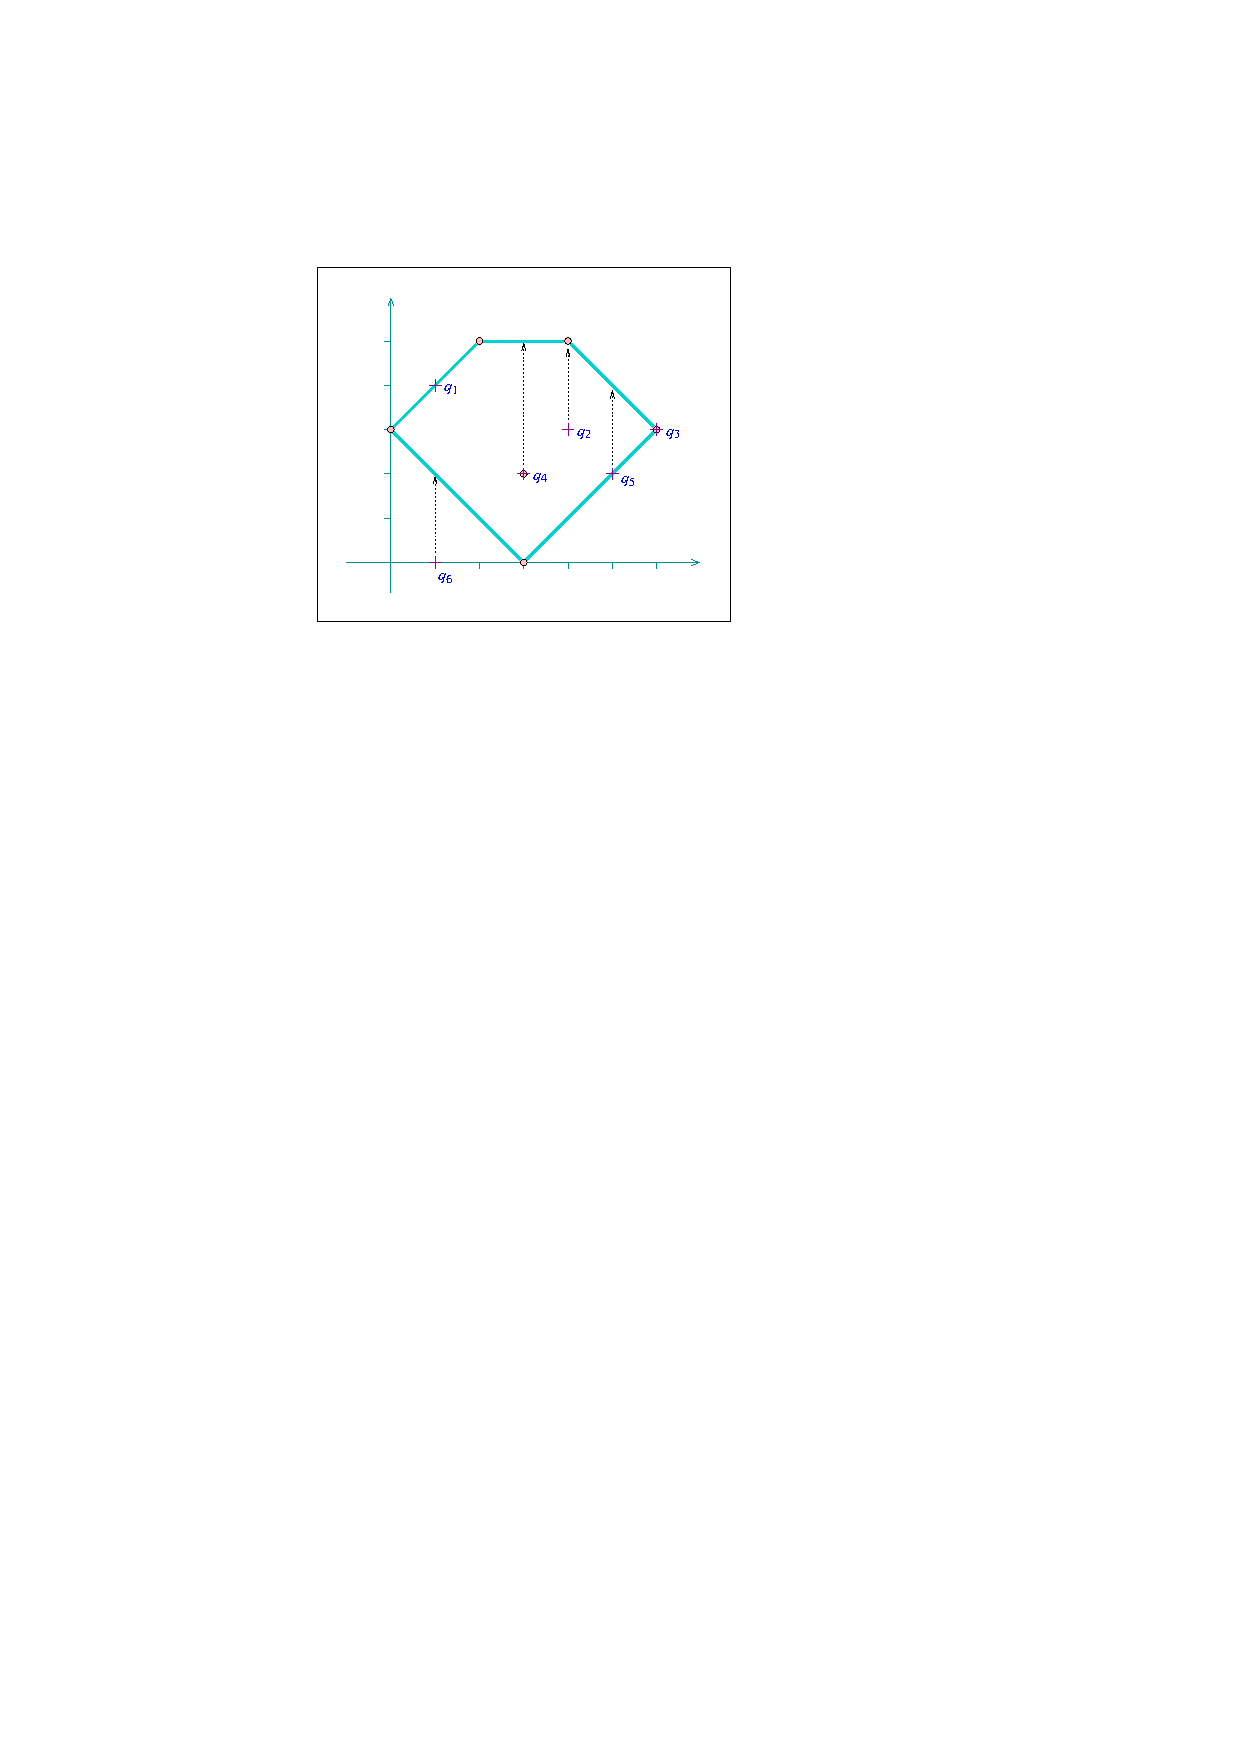
\includegraphics{Arrangement_on_surface_2/fig/ex_5}
  \end{center}
\end{ccTexOnly}
\begin{ccHtmlOnly}
  <p><center>
  <img src="./fig/ex_5.gif" border=0 alt="Example 5">
  </center>
\end{ccHtmlOnly}
\caption{The arrangement of line segments, as constructed in
\ccc{point_location.cpp}, \ccc{vertical_ray_shooting.cpp}, and
\ccc{batched_point_location.cpp}. The
arrangement vertices are drawn as small discs, while the query
points $q_1, \ldots, q_6$ are marked with crosses.\label{arr_fig:ex_5}}
\end{figure}

The following program constructs a simple arrangement of five line
segments that form a pentagonal face, with a single isolated
vertex in its interior, as depicted in Figure~\ref{arr_fig:ex_5}
(the arrangement construction is performed by the function
\ccc{construct_segment_arr()} whose listing is omitted here and
can be found in \ccc{point_location_utils.h}).
It then employs the naive and the landmark strategies to issue
several point-location queries on this arrangement:

\ccIncludeExampleCode{Arrangement_on_surface_2/point_location_example.cpp}

Note that the program uses the auxiliary
\ccc{point_location_query()} function template to nicely print the
result of each query. This function can be found in the header file
\ccc{point_location_utils.h}.

\subsection{Vertical Ray Shooting\label{arr_ssec:ray_shoot}}
%---------------------------------

Another important query issued on arrangements is the vertical
ray-shooting query: Given a query point, which arrangement feature
do we encounter if we shoot a vertical ray emanating upward (or
downward) from this point? In the general case the ray hits an
edge, but it is possible that it hits a vertex, or that the
arrangement does not have any feature lying directly above (or
below) the query point.

All point-location classes listed in the previous section are also models
of the \ccc{ArrangementVerticalRayShoot_2} concept. That is, they all
have member functions called \ccc{ray_shoot_up(q)} and
\ccc{ray_shoot_down(q)} that accept a query point $q$ and output a
\cgal\ \ccc{Object}. This can be assigned to either a
\ccc{Halfedge_const_handle} or to a \ccc{Vertex_const_handle}.
Alternatively, the returned value is a \ccc{Face_const_handle}
for the unbounded face of the arrangement, in case there is no edge
or vertex lying directly above (or below) $q$.

The following function template, \ccc{vertical_ray_shooting_query()},
which also located in the header file \ccc{point_location_utils.h},
accepts a vertical ray-shooting
object, whose type can be any of the models to the
\ccc{ArrangementVerticalRayShoot_2} concept and prints out the
result of the upward vertical ray-shooting operations from a given
query point. The ray-shooting object \ccc{vrs} is assumed to be
already associated with an arrangement:

\begin{alltt}
template <class VerticalRayShoot>
void vertical_ray_shooting_query
    (const VerticalRayShoot& vrs,
     const typename VerticalRayShoot::Arrangement_on_surface_2::Point_2& q)
\{
  // Perform the point-location query.
  CGAL::Object    obj = vrs.ray_shoot_up (q);

  // Print the result.
  typedef typename VerticalRayShoot::Arrangement_on_surface_2  Arrangement_on_surface_2;

  typename Arrangement_on_surface_2::Vertex_const_handle    v;
  typename Arrangement_on_surface_2::Halfedge_const_handle  e;
  typename Arrangement_on_surface_2::Face_const_handle      f;

  std::cout << "Shooting up from " << q << " : ";
  if (CGAL::assign (e, obj)) \{
    // We hit an edge:
    std::cout << "hit an edge: " << e->curve() << std::endl;
  \}
  else if (CGAL::assign (v, obj)) \{
    // We hit a vertex:
    if (v->is_isolated())
      std::cout << "hit an isolated vertex: " << v->point() << std::endl;
    else
      std::cout << "hit a vertex: " << v->point() << std::endl;
  \}
  else if (CGAL::assign (f, obj)) \{
    // We did not hit anything:
    CGAL_assertion (f->is_unbounded());

    std::cout << "hit nothing." << std::endl;
  \}
  else \{
    CGAL_assertion_msg (false, "Invalid object.");
  \}
\}
\end{alltt}

The following program uses the auxiliary function listed above to
perform vertical ray-shooting queries on an arrangement.
The arrangement and the query points are exactly the same as in
\ccc{point_location_example.cpp} (see Figure~\ref{arr_fig:ex_5}):

\ccIncludeExampleCode{Arrangement_on_surface_2/vertical_ray_shooting.cpp}

The number type we use in this example is \cgal's built-in
\ccc{MP_Float} type which is a floating-point number with an
unbounded mantissa and a 32-bit exponent. It supports construction from an
integer or from a machine \ccc{float} or \ccc{double} and performs additions,
subtractions and multiplications in an exact number.

\subsection{Batched Point-Location\label{arr_ssec:batched_pl}}
%----------------------------------

Suppose that at a given moment our application has to issue a
relatively large number $m$ of point-location queries on a
specific arrangement instance. It is possible of course to define
a point-location object and to issue separate queries on the
arrangement. However, as explained in Section~\ref{arr_ssec:pl},
choosing a simple point-location strategy (either the naive or
the walk strategy) means inefficient queries, while the more
sophisticated strategies need to construct auxiliary structures
that incur considerable overhead in running time.

On the other hand, the arrangement package includes a free
\ccc{locate()} function that accepts an arrangement a range of
query points as its input and sweeps through the arrangement to
locate all query points in one pass. The function outputs the query
results as pairs, where each pair is comprised of a query point
and a \cgal\ \ccc{Object} that represents the cell containing the
point (see Section~\ref{arr_ssec:pl}). The output pairs are
sorted in increasing $xy$-lexicographical order of the query point.

The batched point-location operation can be performed in
$O\left((m+N)\log{(m+N)}\right)$ time, where $N$ is the number of
edges in the arrangement. This means that when the number $m$ of
point-location queries is of the same order of magnitude as $N$,
this operation is more efficient than issuing separate queries.
This suggestion is also backed up by experimental results.
Moreover, the batched point-location operation is also
advantageous as it does not have to construct and maintain
additional data structures.

The following program issues a batched point-location query, which
is essentially equivalent to the six separate queries performed in
\ccc{point_location_example.cpp} (see Section~\ref{arr_ssec:pl}):

\ccIncludeExampleCode{Arrangement_on_surface_2/batched_point_location.cpp}
